%!TEX TS-program = xelatex

\documentclass[t]{beamer}

\usetheme{Hannover}
\usecolortheme{rose}

%%% Работа с русским языком
\usepackage[english,russian]{babel}   %% загружает пакет многоязыковой вёрстки
\usepackage{fontspec,xltxtra,xunicode}      %% подготавливает загрузку шрифтов Open Type, True Type и др.
%\defaultfontfeatures{Ligatures={TeX},Renderer=Basic}  %% свойства шрифтов по умолчанию
\setmainfont[Ligatures={TeX,Historic},
SmallCapsFont={Brill},
SmallCapsFeatures={Letters=SmallCaps}]{Brill} %% задаёт основной шрифт документа
\setsansfont{Brill}                    %% задаёт шрифт без засечек
\setmonofont[Ligatures=NoCommon]{DejaVu Sans}
\newfontfamily\SYM{Brill}
\usepackage{indentfirst}
%%% Дополнительная работа с математикой
\usepackage{amsmath,amsfonts,amssymb,amsthm,mathtools} % AMS
\usepackage{icomma} % "Умная" запятая: $0,2$ --- число, $0, 2$ --- перечисление

%%% Работа с картинками
\usepackage{wrapfig} % Обтекание рисунков текстом
\usepackage{rotating}
\usepackage{fixltx2e}
\usepackage{hhline}
\usepackage{lscape}

%%% Работа с таблицами
\usepackage{array,tabularx,tabulary,booktabs} % Дополнительная работа с таблицами
\usepackage{longtable}  % Длинные таблицы
\usepackage{multirow} % Слияние строк в таблице

\usepackage{multicol} % Несколько колонок

%%% Страница
%\usepackage{fancyhdr} % Колонтитулы
% 	\pagestyle{fancy}
 	%\renewcommand{\headrulewidth}{0pt}  % Толщина линейки, отчеркивающей верхний колонтитул
% 	\lfoot{Нижний левый}
% 	\rfoot{Нижний правый}
% 	\rhead{Верхний правый}
% 	\chead{Верхний в центре}
% 	\lhead{Верхний левый}
%	\cfoot{Нижний в центре} % По умолчанию здесь номер страницы

\usepackage{setspace} % Интерлиньяж
%\onehalfspacing % Интерлиньяж 1.5
%\doublespacing % Интерлиньяж 2
\singlespacing % Интерлиньяж 1

\usepackage{subfig} % подкартинки
\usepackage{lastpage} % Узнать, сколько всего страниц в документе.
\usepackage{soul} % Модификаторы начертания
\usepackage{bbding}
\usepackage{hyperref}
\usepackage{tikz} % Работа с графикой
\usepackage{pgfplots}
\usepackage{pgfplotstable}
\usepackage{verbatim}

\usepackage{attachfile2}
 \attachfilesetup{appearance=true,
color=0 0 0
 }
\usepackage{alltt}

%%% Лингвистические пакеты
%\usepackage{savetrees} % пакет, который экономит место
\usepackage{forest} % для рисования деревьев
\usepackage{vowel} % для рисования трапеций гласных
\usepackage{natbib}
\bibpunct[: ]{[}{]}{;}{a}{}{,}
\usepackage[nogroupskip,nopostdot, nonumberlist]{glossaries}
%\usepackage{glossary-mcols} 
%\setglossarystyle{mcolindex}
\usepackage{philex} % пакет для примеров
\newcommand{\mytem}{\item[$\circ$]}
\addto\captionsrussian{
\renewcommand{\refname}{}}

\newcommand{\apostrophe}{\XeTeXglyph\XeTeXcharglyph"0027\relax}
\usetikzlibrary{patterns}

\usepackage{ulem}
\usepackage{subfig}
\setbeamercolor{alerted text}{fg=red!13!blue}
\setbeamersize{text margin left=4mm,text margin right=1mm} 
\setbeamertemplate{navigation symbols}{
	\usebeamerfont{footline}%
    \usebeamercolor[fg]{footline}%
    \hspace{1em}%
    {{\small презентация доступна: \href{http://goo.gl/AdqRQl}{\textbf{http://goo.gl/AdqRQl}}}
    \hspace{4.3cm}
    \insertframenumber/\inserttotalframenumber\vspace{0.5mm}}}
\newcommand{\mcrot}[4]{\multicolumn{#1}{#2}{\rlap{\rotatebox{#3}{#4}~}}} 
% начало
\title[]{Корреляции и другие связи переменных. Регрессионный анализ}
\author[]{Г. Мороз}
\date{}
\begin{document}
\frame{\titlepage}
\section{связи переменных}
\begin{frame}{Связаны ли одни переменные с другими?}
\begin{itemize}
\mytem две количественные переменные \hfill \alert{как связаны?}
\begin{itemize}
\item[$\Rightarrow$] коэффициенты корреляции Пирсона, Спирмана, Кенделла
\end{itemize}
\mytem две качественные переменные 
\begin{itemize}
\item[$\Rightarrow$] \scriptsize\verb"aggregate()"\normalsize, χ², тест Фишера  \hfill \alert{связи нет?}
\end{itemize}
\mytem одна количественная и одна качественная переменная
\begin{itemize}
\item[$\Rightarrow$] ANOVA  \hfill \alert{связи нет?}
\end{itemize}
\end{itemize}
\vfill
К сожалению, слово \textit{"корреляция"} и его однокоренные в языке используется куда шире (примеры из НКРЯ):\\
\small
\textit{"…существует четкая корреляция между континентом проведения соревнований и результатом…"}\\
\textit{"…существует прямая корреляция между владением азиатскими «тональными» языками и хорошим музыкальным слухом…"}\\
\textit{"…прямая корреляция количества крыс в доме зависит от наличия мусоропровода и его состояния…"}\\
\normalsize
В статистике \textbf{корреляция} — это отношение между \textbf{числовыми} переменными.
\end{frame}
\subsection{корреляции}
\begin{frame}{Коэффициент корреляции Пирсона}
Коэффициент корреляции позволяет показать степень взаимосвязи между двумя величинами. Коэффициент корреляции изменяется от -1 до 1, где 0 обозначает отсутствие взаимосвязи, положительное значение коэффициента указывает на прямую взаимосвязь (чем больше $x$, тем больше $y$), а отрицательное — на обратную (чем больше $x$, тем меньше $y$).\\
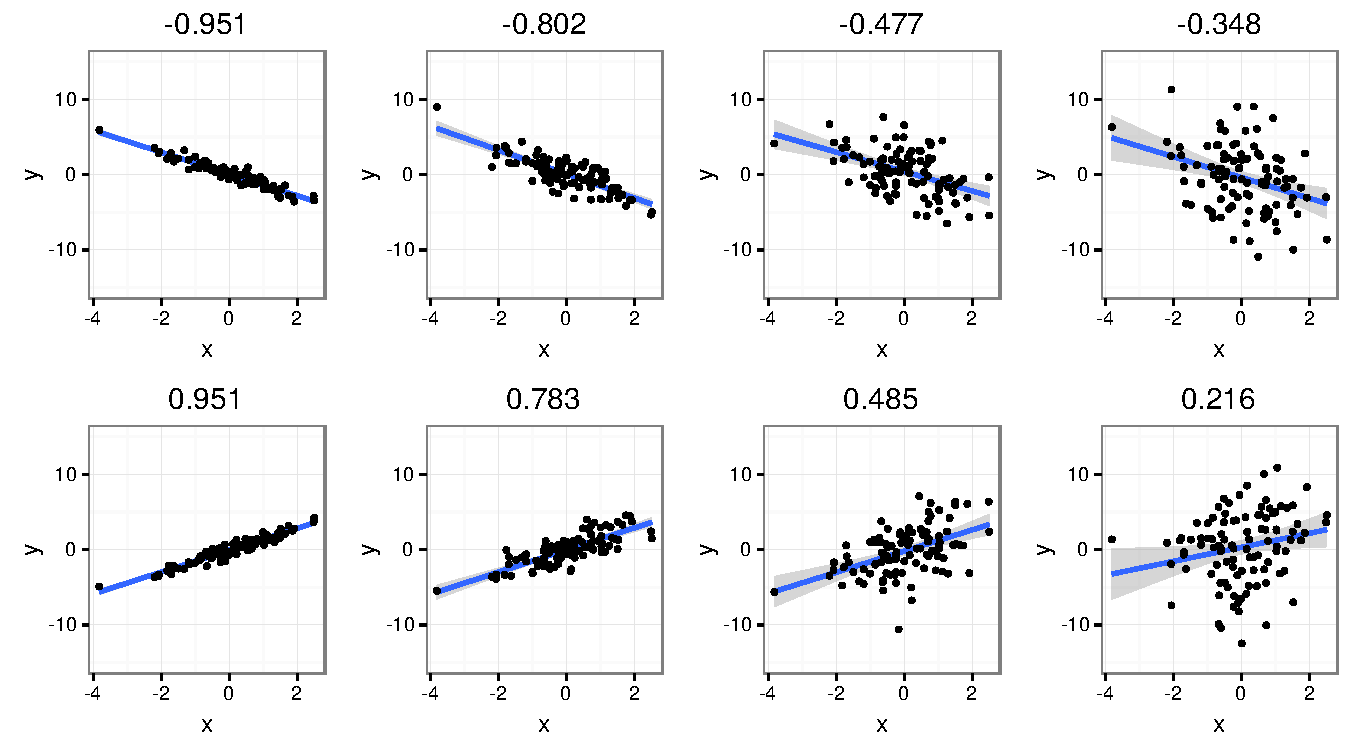
\includegraphics[width=0.9\linewidth]{correlation.pdf}\\
\end{frame}
\begin{frame}{Коэффициент корреляции Пирсона}
Значение коэффициента корреляции Пирсона зависит от удаленности точек от регрессионной прямой и \textbf{никак} не зависит от наклона данной прямой. См. примеры из \href{https://upload.wikimedia.org/wikipedia/commons/d/d4/Correlation_examples2.svg}{\alert{Википедии}}.
\scriptsize
\begin{alltt}
x <- c(2, 8, 3, 7, 11, 3)\\
y <- c(12, 7, 10, 8, 5, 11)\\
\alert{cor(x, y) \hfill \# по умолчанию считается коэффициент корреляции Пирсона}\\
\alert{cor.test(x, y) \hfill \# H$_0$: коэффициент равен нулю} \medskip\\
Pearson's product-moment correlation\\
data:  x and y\\
t = -12.03, df = 4, p-value = 0.0002737 \\
alternative hypothesis: true correlation is not equal to 0\\
95 percent confidence interval:\\
 -0.9985831 -0.8770124 \hfill доверительный интервал для коэффициента\\
sample estimates:\\
-0.9864609 \hfill коэффициент корреляции
\end{alltt}
\normalsize
\vfill
тип данных: числовой\\
параметрический (требует линейности связи)\\~
\end{frame}
\begin{frame}{Коэффициенты корреляции Спирмана, Кенделла}
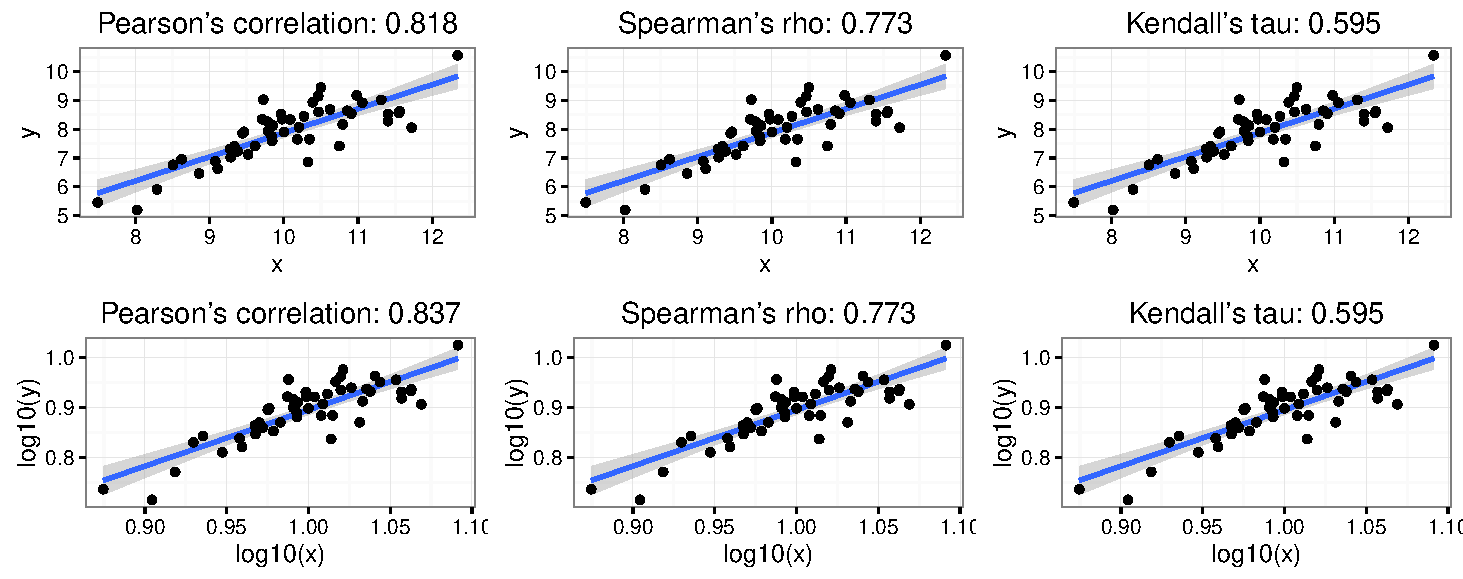
\includegraphics[width=\linewidth]{correlation2.pdf}\\
\scriptsize
\begin{alltt}
x <- c(2, 8, 3, 7, 11, 3)\\
y <- c(12, 7, 10, 8, 5, 11)\\
\alert{cor(x, y, method = "spearman") \hfill \# коэффициент корреляции Спирмана}\\
\alert{cor.test(x, y, method = "spearman")}\\
\alert{cor(x, y, method = "kendall") \hfill \# коэффициент корреляции Кенделла}\\
\alert{cor.test(x, y, method = "kendall")}
\end{alltt}
\normalsize
\vfill
тип данных: числовой\\
непараметрический\\~
\end{frame}
\begin{frame}{Корреляционная матрица: PerformanceAnalytics}
\scriptsize
\begin{alltt}
library(PerformanceAnalytics)\\
chart.Correlation(mydata)\\
chart.Correlation(mydata, method = "spearman")\\
chart.Correlation(mydata, method = "kendall")
\end{alltt}
\normalsize
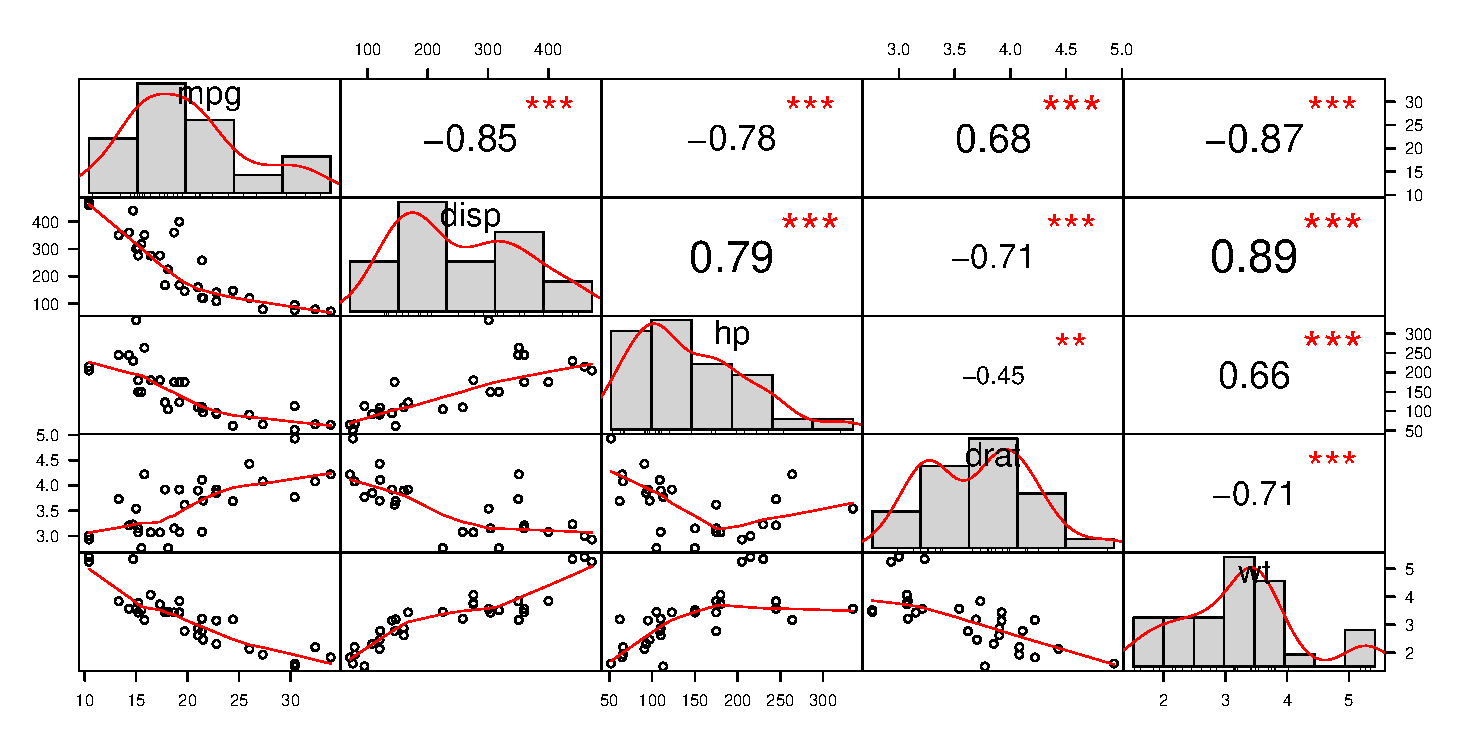
\includegraphics[width=\linewidth]{cormatrix1.pdf}
\end{frame}
\begin{frame}{Корреляционная матрица: ellipse}
\href{https://hlplab.wordpress.com/2012/03/20/correlation-plot-matrices-using-the-ellipse-library/}{\alert{Здесь пример}} использованием пакета \scriptsize\verb"ellipse"\normalsize.\\
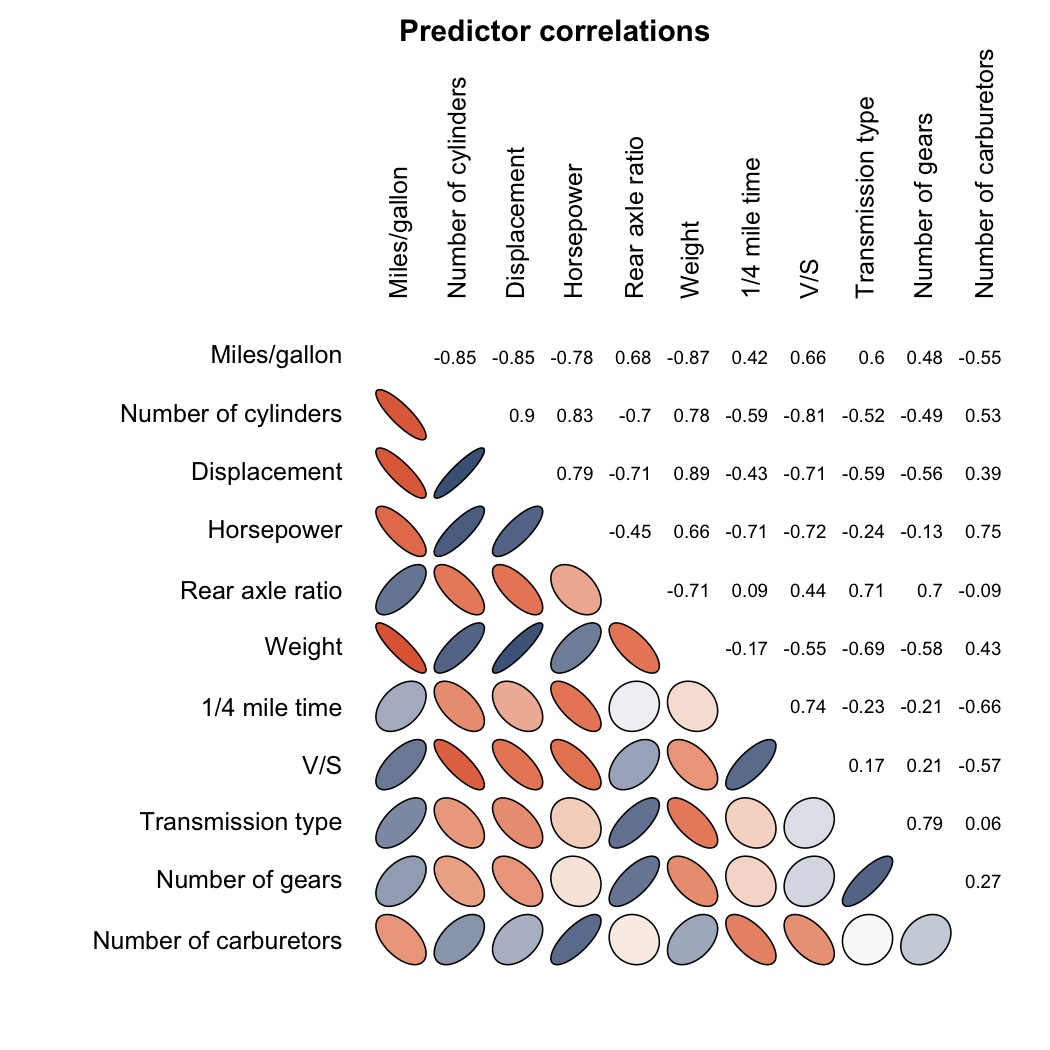
\includegraphics[width=0.70\linewidth]{plotcor.jpg}
\end{frame}
\subsection{aggregate()}
\begin{frame}{aggregate()}
В работе \citep{cedergren73} ис следовались отпадение согласного [s] в конце слова в речи жителей Панамы. При каких условиях выпадение [s] происходит чаще всего?
\scriptsize
\begin{alltt}
\alert{tail(dat)}\\
\begin{tabular}{rrrrr}
 & s.deletion & gramm.cat & phon.cont & social \\
8841 & not deleted & noun & pause & 2 \\
8842 & not deleted & noun & pause & 2 \\
8843 & not deleted & noun & pause & 3 \\
8844 & not deleted & noun & pause & 3 \\
8845 & not deleted & noun & pause & 4 \\ 
8846 & not deleted & noun & pause & 4 \\ 
\end{tabular}
\\
\alert{sapply(dat, table)}\\
\$s.deletion\\
\begin{tabular}{rr}
deleted & not deleted \\
5091 & 3755 \\
\end{tabular}\\
\$gramm.cat\\
\begin{tabular}{rrrrr}
adjective & determiner & noun & separate morpheme & verb \\
609 & 1393 & 2268 & 4460 & 116 \\
\end{tabular}\\
\$phon.cont\\
\begin{tabular}{rrr}
consonant & pause & vowel \\
5600 & 1304 & 1942 \\
\end{tabular}\\
\$social\\
\begin{tabular}{rrrr}
1 & 2 & 3 & 4 \\
579 & 2547 & 2385 & 3335 \\
\end{tabular}
\end{alltt}
\normalsize
\end{frame}
\begin{frame}
\scriptsize
\begin{alltt}
\alert{aggregate(s.deletion\textasciitilde gramm.cat, \hfill \# формула\\
data = a, \hfill \# данные\\
summary)\hfill \# функция\\}
\begin{tabular}{rrrr}
\multicolumn{1}{l}{} & gramm.cat & \multicolumn{1}{l}{s.deletion.no} & \multicolumn{1}{l}{s.deletion.yes} \\ 
1 & adjective & 311 & 298 \\ 
2 & determiner & 789 & 604 \\ 
3 & noun & 674 & 1594 \\ 
4 & separate morpheme & 1904 & 2556 \\ 
5 & verb & 77 & 39 \\ 
\end{tabular}
\\
\alert{aggregate(s.deletion\textasciitilde gramm.cat + phon.cont, \hfill \# формула\\
data = a, \hfill \# данные\\
summary)\hfill \# функция\\}
\begin{tabular}{rrrrr}
 & gramm.cat & phon.cont & s.deletion.no & s.deletion.yes \\
1 & adjective & consonant & 261 & 205\\ 
2 & determiner & consonant & 678 & 524 \\ 
3 & noun & consonant & 418 & 733 \\ 
4 & separate morpheme & consonant & 1361 & 1355 \\ 
5 & verb & consonant & 42 & 23 \\ 
6 & adjective & pause & 22 & 48 \\ 
7 & noun & pause & 132 & 485 \\ 
8 & separate morpheme & pause & 146 & 471 \\ 
9 & adjective & vowell & 28 & 45 \\ 
10 & determiner & vowell & 111 & 80 \\ 
11 & noun & vowell & 124 & 376 \\ 
12 & separate morpheme & vowell & 397 & 730 \\ 
13 & verb & vowell & 35 & 16 \\ 
\end{tabular}
\end{alltt}
\normalsize
\end{frame}
\begin{frame}
\scriptsize
\begin{alltt}
b <- aggregate(s.deletion\textasciitilde gramm.cat, \\
                    data = a, \\
                    summary) \\
\alert{\# лучше смотреть на соотношения в процентах}\\
\alert{\# apply(df, 1, FUN) применяет функцию FUN к каждой строчке df}\\
b\$prop.no <- apply(b[,length(b)], 1, prop.table)[1,]\\
b\$prop.yes <- apply(b[,length(b)-1], 1, prop.table)[2,]\\
b\\
\begin{tabular}{rrrrrr}
\multicolumn{1}{l}{} & gramm.cat & \multicolumn{1}{l}{s.delet.no} & \multicolumn{1}{l}{s.delet.yes} & \alert{prop.no} & \alert{prop.yes} \\ 
1 & adjective & 311 & 298 & \alert{0.51} & \alert{0.49} \\ 
2 & determiner & 789 & 604 & \alert{0.57} & \alert{0.43} \\ 
3 & noun & 674 & 1594 & \alert{0.30} & \alert{0.70} \\ 
4 & separate morpheme & 1904 & 2556 & \alert{0.43} & \alert{0.57} \\ 
5 & verb & 77 & 39 & \alert{0.66} & \alert{0.34} \\ 
\end{tabular}
\end{alltt}
\normalsize
\end{frame}
\begin{frame}{Correlation does not imply causation!}
Это говорят на всех курсах по статистике. Примером могут служить \href{http://tylervigen.com/spurious-correlations}{\alert{сайт}} и сделанная на его основе \href{http://www.indiebound.org/book/9780316339438}{\alert{книга}} \textit{Spurious correlations}.
\vfill
Если есть корреляция между двумя переменными $a$ и $b$, то может быть один из следующих вариантов:
\begin{itemize}
\mytem $a$ вызывает $b$
\mytem $b$ вызывает $a$
\mytem $a$ вызывает $b$, а $b$ вызывает $a$
\mytem $a$ вызывает $c$, а $c$ вызывает $b$
\mytem $c$ вызывает $a$ и $b$, но $a$ и $b$ не связаны
\mytem $a$ и $b$ не связаны
\end{itemize}
\vfill
Однако часто приводят примеры лишь на последнее. Кстати, вы знали, что \href{https://upload.wikimedia.org/wikipedia/commons/e/e6/PiratesVsTemp.svg}{\alert{количество пиратов влияет на глобальное потепление}}? А еще… чем больше пожарников посылают тушить пожар, тем больше ущерба он наносит.
\end{frame}
\section{регрессии}
\begin{frame}{Статистическая модель}
Когда мы работаем с данными и находим отношения между какими-то из переменных, мы создаем упрощенное представление некоторой системы, которые мы в дальнейшем будем называть \textit{моделью}. Получившаяся модель позволяет нам с некоторой точностью предсказывать некоторый результат на основе той или иной конфигурации параметров модели. Чаще всего в статистические модели закладывается стохастический элемент, т. е. даже в самой простой модели будет случайная переменная, которую еще называют \alert{остатками модели}:  $$y=4+\alert{\mbox{ε}_i}$$
Таким образом любое статистическое моделирование — это поиск наилучшей аппроксимация закона распределения исследуемой переменной, так чтобы обеспечить минимум \alert{средней ошибки ε$_i$}.
\end{frame}
\section{линейная регрессия}
\begin{frame}{Линейная регрессия}
В работе исследовалась зависимость средней значения частоты основного тона от возраста (мужчины и женщины следует считать отдельно). Какие коэффициенты получит регрессионные линии и сколько процентов дисперсии объяснят наши модели, если мы предположим линейную зависимость между переменными?\pause
\vfill
$$y=\mbox{β}_0+\mbox{β}_1\cdot x+\mbox{ε}_i,$$
где $x$  — предиктор, $\mbox{β}_0$  — свободный член, $\mbox{β}_1$  — угловой коэффициент, $\mbox{ε}_i$  — средняя ошибка.
\vfill

\end{frame}
\begin{frame}{Линейная регрессия: строим модель}
\scriptsize
\begin{alltt}
\alert{summary(df)}\\
\begin{tabular}{lllll}
\multicolumn{1}{c}{sex} & \multicolumn{2}{c}{age} & \multicolumn{2}{c}{pitch} \\
f:20                    & Min.        & :23.00    & Min.         & :139.3     \\
m:20                    & 1st Qu.     & :46.50    & 1st Qu.      & :154.3     \\
                        & Median      & :62.50    & Median       & :158.8     \\
                        & Mean        & :59.12    & Mean         & :159.3     \\
                        & 3rd Qu.     & :71.25    & 3rd Qu.      & :162.4     \\
                        & Max.        & :83.00    & Max.         & :176.4    
\end{tabular}
\bigskip \\
dfm <- subset(df, sex=="m") \hfill \# сгруппируем по полу\\
dff <- subset(df, sex=="f")  \hfill \# сгруппируем по полу \bigskip \\
fit.f <- \alert{lm(pitch\textasciitilde age, dff)} \hfill \# cтроим регрессию\\
fit.m <- \alert{lm(pitch\textasciitilde age, dfm)} \hfill \# cтроим регрессию\\
\end{alltt}
\normalsize
\vfill
В случае, если в задаче требуется исключить свободный член, то в формулу нужно добавить \scriptsize\verb"-1"\normalsize:
\scriptsize
\begin{alltt}
fit.m2 <- \alert{lm(pitch\textasciitilde age - 1, dfm)} \hfill \# исключаем свободный член\\
\end{alltt}
\normalsize
\end{frame}
\begin{frame}{Линейная регрессия: анализ результатов}
\scriptsize
\begin{alltt}
fit.f <- \alert{lm(pitch\textasciitilde age, dff)} \hfill \# cтроим регрессию по данным женщин\\
\alert{summary(fit.f)}\bigskip\\
Call:\\
lm(formula = pitch \textasciitilde  age, data = dff)\hfill \# формула, вдруг забыли \bigskip\\
Residuals: \hfill \# распределение остатков\\
\begin{tabular}{rrrrr}
Min & 1Q & Median &3Q & Max \\
-2.33997 & -0.62471 & -0.06519  & 0.70728 &  1.66992  \\
\end{tabular}
\bigskip\\
Coefficients:\hfill \# коэффициенты модели\\
\begin{tabular}{llllllr}
					 	& Estimate		& Std. Error	& t value	&Pr(>|t|)	&  		& \\
(Intercept)		& 189.87935  &  1.00978 & 188.04  & < 2e-16 & *** 	& \alert{\# $\mbox{β}_0$}\\
age   				& -0.39820  &  0.01605 & -24.81 & 2.27e-15 &***	&  \alert{\# $\mbox{β}_1$}\\
\end{tabular}
\\
---\\
Signif. codes:  0 ‘***’ 0.001 ‘**’ 0.01 ‘*’ 0.05 ‘.’ 0.1 ‘ ’ 1\medskip\\
Residual standard error: 1.134 on 18 degrees of freedom\\
Multiple R-squared:  0.9716,	\alert{Adjusted R-squared:   0.97} \\
F-statistic: 615.5 on 1 and 18 DF,  p-value: 2.267e-15\\
\end{alltt}
\normalsize
\alert{Что означают p-values?}
\end{frame}

\begin{frame}{Линейная регрессия: анализ результатов}
\scriptsize
\begin{alltt}
fit.m <- \alert{lm(pitch\textasciitilde age, dfm)} \hfill \# cтроим регрессию по данным женщин\\
\alert{summary(fit.m)}\bigskip\\
Call:\\
lm(formula = pitch \textasciitilde  age, data = dfm)\hfill \# формула, вдруг забыли \bigskip\\
Residuals: \hfill \# распределение остатков\\
\begin{tabular}{rrrrr}
Min & 1Q & Median &3Q & Max \\
-1.87771 & -0.54867 & 0.05222 & 0.88251 & 1.79433 \\
\end{tabular}
\bigskip\\
Coefficients:\hfill \# коэффициенты модели\\
\begin{tabular}{llllllr}
					 	& Estimate		& Std. Error	& t value	&Pr(>|t|)	&  		& \\
(Intercept)		& 130.07015	&   0.90750		&  143.33		&  < 2e-16 	& *** 	& \alert{\# $\mbox{β}_0$}\\
age   				& 0.39790		& 0.01534		& 25.94		& 1.04e-15	&***	&  \alert{\# $\mbox{β}_1$}\\
\end{tabular}
\\
---\\
Signif. codes:  0 ‘***’ 0.001 ‘**’ 0.01 ‘*’ 0.05 ‘.’ 0.1 ‘ ’ 1\medskip\\
Residual standard error: 0.9985 on 18 degrees of freedom\\
Multiple R-squared:  0.974,	\alert{Adjusted R-squared:  0.9725} \\
F-statistic:   673 on 1 and 18 DF,  p-value: 1.036e-15\\
\end{alltt}
\normalsize
\alert{Что означают p-values?}
\end{frame}
\begin{frame}{Линейная регрессия: визуализация, R-base}
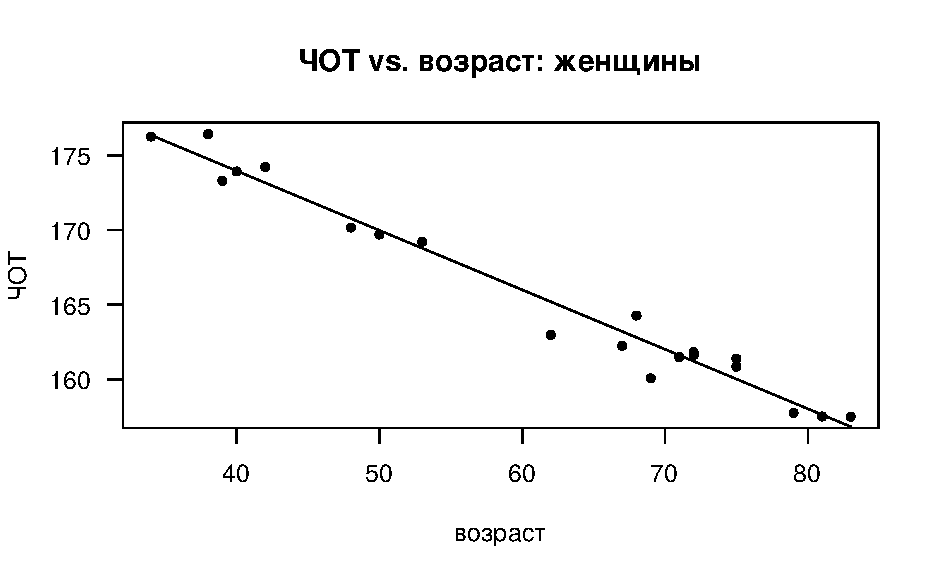
\includegraphics[width=\linewidth]{linearbaser.pdf}
\scriptsize
\begin{alltt}
fit.f <- lm(pitch\textasciitilde  age, dff)\\
plot(dff\$age, dff\$pitch)\\
lines(dff\$age, \alert{fit.f\$fitted.values})
\end{alltt}
\normalsize
\end{frame}
\begin{frame}{Линейная регрессия: визуализация, ggplot2}
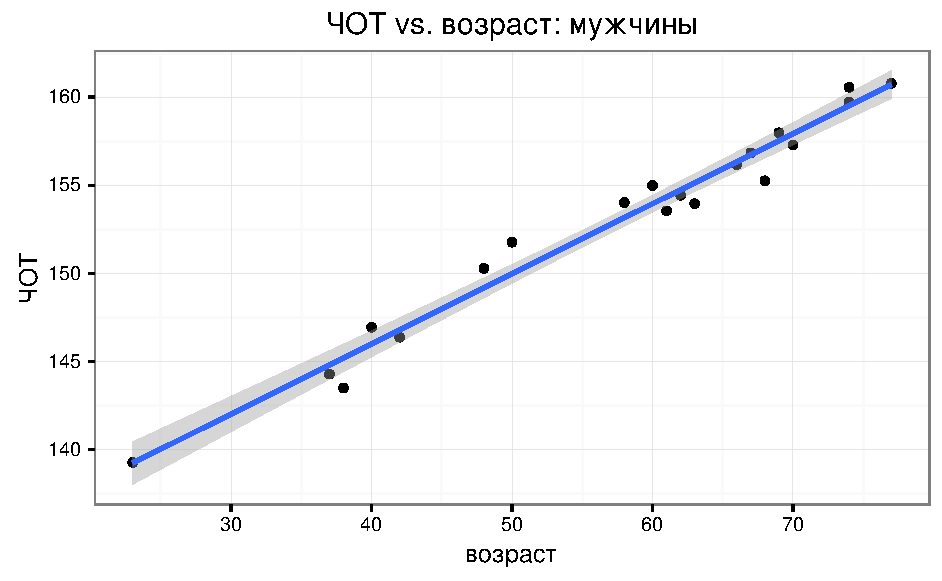
\includegraphics[width=0.95\linewidth]{linearggplot.pdf}
\scriptsize
\begin{alltt}
library(ggplot2)\\
ggplot(dfm, aes(x=age, y = pitch))+\\
  geom\_point()+\\
\alert{geom\_smooth(method = "lm") \hfill \# уже встроена линейная регрессия}\\
\end{alltt}
\normalsize
\end{frame}
\begin{frame}{Линейная регрессия: доверительный интервал}
Так как регрессия строится по выборочным данным, мы не знаем, как бы проходила линия, если бы мы взяли другую выборку. Т. е. значения коэффициентов $\mbox{β}_0$ и $\mbox{β}_1$, вычисленные функцией \scriptsize\verb"lm()"\normalsize, являются лишь некоторым приближением к коэффициентам регрессии, которая бы описывала параметры генеральной совокупности.
\vfill
В вязи с этим стоит строить доверительный интервал регрессии, что позволяет делать команда \scriptsize\verb"predict()"\normalsize.
\scriptsize
\begin{alltt}
head(\alert{predict(fit.f, interval = "conf")})\\
\begin{tabular}{rrrr}
 & fit & lwr& upr \\
1 & 158.4218 & 157.6118    & 159.2319 \\
2 & 162.8020 & 162.2180 & 163.3859 \\
3 & 162.4038 & 161.8052 & 163.0023 \\
4 & 163.2002 & 162.6292 & 163.7711 \\
5 & 161.6074 & 160.9752  & 162.2396 \\
6 & 161.2092 & 160.5582 & 161.8602 \\
\end{tabular}
\end{alltt}
\normalsize
\end{frame}
\begin{frame}{Линейная регрессия: CI, R-base}
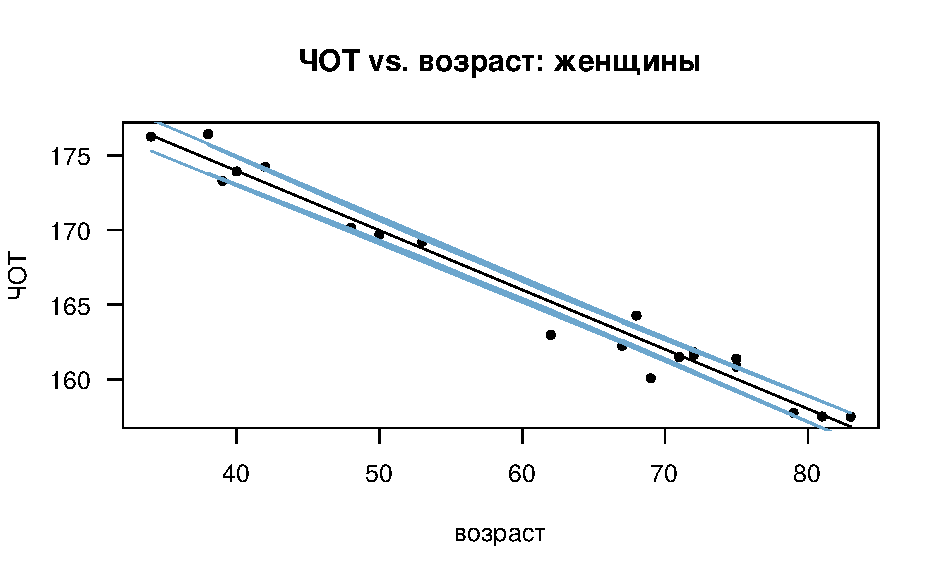
\includegraphics[width=0.9\linewidth]{regressionci.pdf}
\scriptsize
\begin{alltt}
fit.f <- lm(pitch\textasciitilde  age, dff) \hfill \# строим модель\\
\alert{pred.f} <- \alert{predict(fit.f, interval = "conf")}\hfill \# строим границы\\
plot(dff\$age, dff\$pitch)\\
lines(dff\$age, \alert{pred.f[,1]})\hfill \# линия регрессии\\
lines(dff\$age, \alert{pred.f[,2]}, col = "skyblue3") \hfill \# нижняя гр. CI\\
lines(dff\$age, \alert{pred.f[,3]}, col = "skyblue3") \hfill \# верхняя гр. CI\\
~
\end{alltt}
\normalsize
\end{frame}
\begin{frame}{Линейная регрессия: CI, ggplot2}
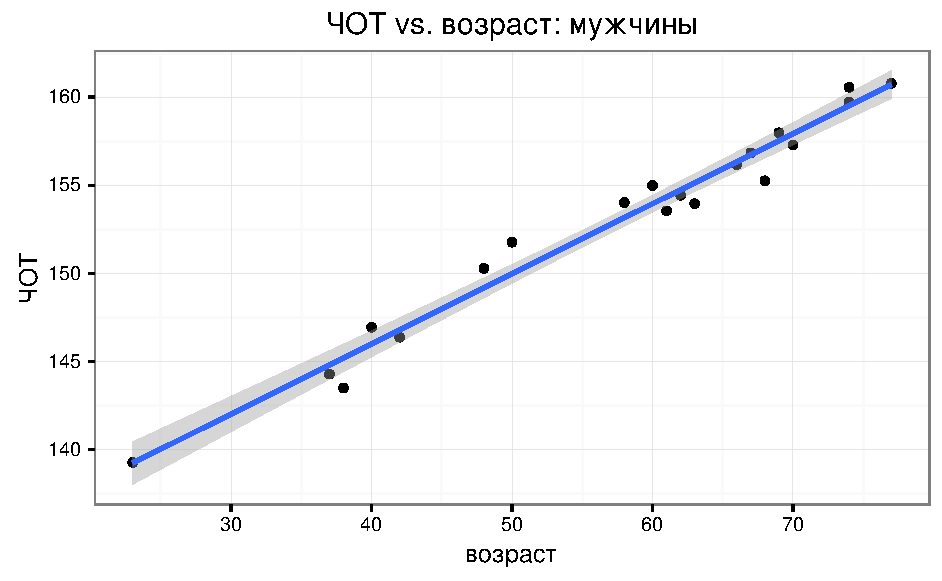
\includegraphics[width=0.95\linewidth]{linearggplot.pdf}
\scriptsize
\begin{alltt}
library(ggplot2)\\
ggplot(dfm, aes(x=age, y = pitch))+\\
  geom\_point()+\\
\alert{geom\_smooth(method = "lm") \hfill \# уже встроен CI}\\
\end{alltt}
\normalsize
\end{frame}
\section{dummy-переменные}
\begin{frame}{dummy-переменные}
В регрессионные модели можно включить и категориальные предикторы. Для этого вводятся фиктивные переменные (dummy variables), принимающие значение либо 1, либо 0. При этом фиктивных переменных должно быть на одну меньше, чем значений, которые принимает категориальные переменные.
\end{frame}
\begin{frame}{dummy-переменные}
Проанализируем \href{http://goo.gl/0btfKa}{\alert{данные}}, содержащих выборку языков с указанием количества согласных и наличия в данном языке абруптивных согласных. На графике представлен результат (можно посмотреть \href{http://goo.gl/JgrU6g}{\alert{более интерактивный вариант}}):\\
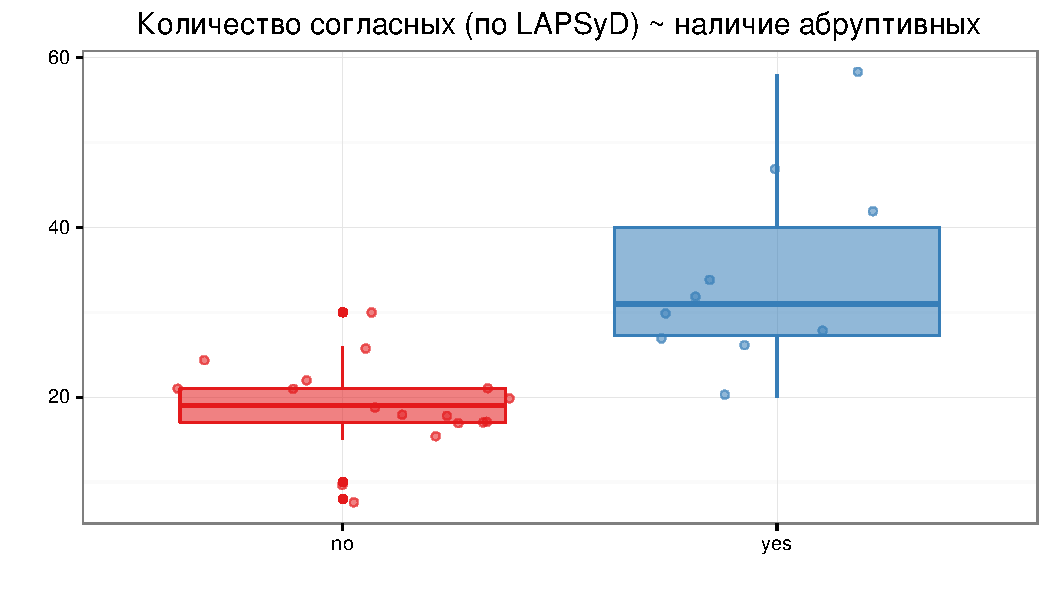
\includegraphics[width=0.99\linewidth]{ejectives.pdf}
\end{frame}
\begin{frame}{dummy-переменные}
\scriptsize
\begin{alltt}
m <- lm(n.cons.lapsyd \textasciitilde\ ejectives, data = ejectives)\\
summary(m)\bigskip\\
Call:\\
lm(formula = n.cons.lapsyd \textasciitilde\ ejectives, data = ejectives)\bigskip\\
Residuals:\\
\begin{tabular}{rrrrr}
Min & 1Q & Median & 3Q & Max \\ 
-14.400 & -4.229 & -1.059 & 2.441 & 23.600 \\
\end{tabular}
\bigskip\\
Coefficients:\\
\begin{tabular}{rrrrrr}
& Estimate & Std.  Error & t & value & Pr(>|t|) \\ 
(Intercept) & 19.059 & 1.953 & 9.758 & 5.25e-10 & *** \\ 
\alert{ejectivesyes} & \alert{15.341} & \alert{3.209} & \alert{4.780} & \alert{6.59e-05} & \alert{***} \\ 
\end{tabular}
\\---\\
Signif. codes:  0 ‘***’ 0.001 ‘**’ 0.01 ‘*’ 0.05 ‘.’ 0.1 ‘ ’ 1\bigskip\\
Residual standard error: 8.053 on 25 degrees of freedom\\
Multiple R-squared:  0.4775,	Adjusted R-squared:  0.4566\\ 
F-statistic: 22.85 on 1 and 25 DF,  p-value: 6.588e-05
\end{alltt}
\normalsize
\end{frame}
\begin{frame}{dummy-переменные}
Естественно в модели переменная может принимать больше двух значений.
\vfill
Регрессионное моделирование, в котором предсказываемая переменная — количественная, а все предикторы — категориальные, называют \alert{ANOVA (Analysis of Variance)}.
\end{frame}
\section{множественная регрессия}
\begin{frame}{А что если количество предикторов больше двух?}
\begin{itemize}
\mytem попарное сравнение \scriptsize\verb"pairs()"\normalsize
\mytem несколько регрессий
\mytem множественная регрессия
\mytem …
\end{itemize}
\end{frame}
\begin{frame}{А что если количество предикторов больше двух?}
\begin{itemize}
\mytem попарное сравнение \scriptsize\verb"pairs()"\normalsize
\end{itemize}
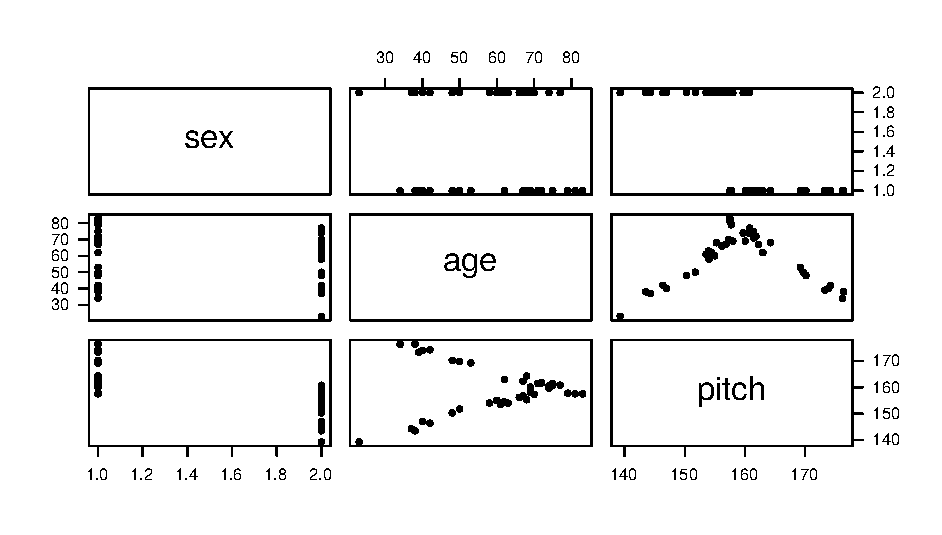
\includegraphics[width=\linewidth]{pairs.pdf}
\end{frame}
\begin{frame}{А что если количество предикторов больше двух?}
\begin{itemize}
\mytem несколько регрессий
\end{itemize}
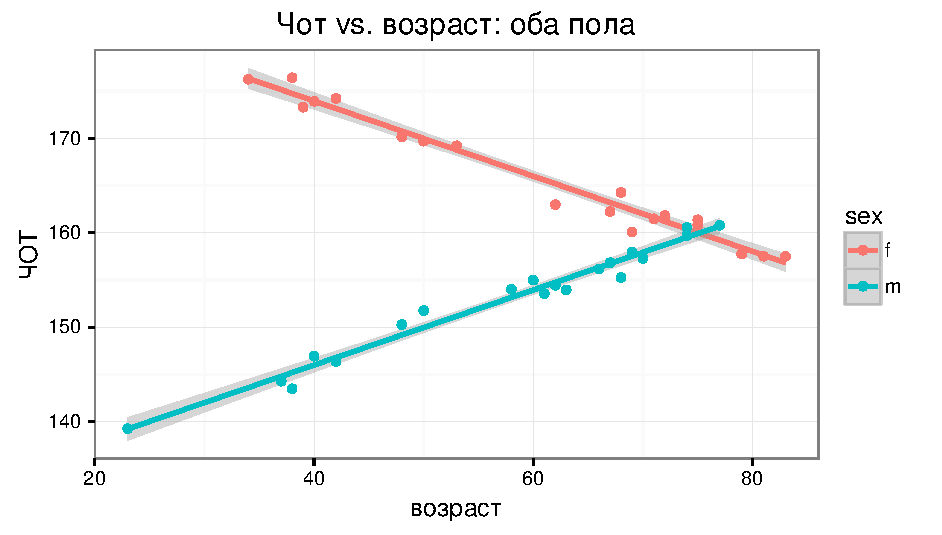
\includegraphics[width=\linewidth]{tworegr.pdf}
\end{frame}
\begin{frame}{Множественная регрессия}
Естественным обобщением линейной регрессии является множественная регрессия, в которой имеется не один предиктор, а несколько:
\vfill
$$y=\mbox{β}_0+\mbox{β}_1\cdot x_1+\mbox{β}_2\cdot x_2 + \dots +\mbox{β}_k\cdot x_k +\mbox{ε}_i,$$
где $x_1, x_2, \dots, x_k$  — предиктор, $\mbox{β}_0$  — свободный член, $\mbox{β}_1, \mbox{β}_2, \dots, \mbox{β}_k$  — коэффициенты регрессии, $\mbox{ε}_i$  — средняя ошибка.
\end{frame}
\section{сравнение моделей}
\begin{frame}{Как сравнить модели?}
Для сравнения моделей используют несколько параметров:
\begin{itemize}
\mytem p-value модели, и p-value коэффициентов регрессии
\mytem R² и adjusted R² — доля дисперсии, объясняемая моделью
\mytem AIC — информационный критерий Акаике (чем меньше, тем лучше)
\mytem BIC — байесовский информационный критерий Шварца (чем меньше, тем лучше)
\mytem результаты перекрестной проверки (cross-validation) — существует много разных техник
\end{itemize}
В работе \citep{stone77}, видимо, показано, что AIC и некоторые методы перекрестной проверки асимптотически эквивалентны.
\end{frame}

\begin{frame}{Как сравнить модели? p-value}
Для сравнения моделей используют несколько параметров:
\begin{itemize}
\mytem p-value модели, и p-value коэффициентов регрессии.
\end{itemize}
\scriptsize
\begin{alltt}
Call:\\
lm(formula = pitch \textasciitilde  age, data = dfm)\hfill \# формула, вдруг забыли \bigskip\\
Residuals: \hfill \# распределение остатков\\
\begin{tabular}{rrrrr}
Min & 1Q & Median &3Q & Max \\
-1.87771 & -0.54867 & 0.05222 & 0.88251 & 1.79433 \\
\end{tabular}
\bigskip\\
Coefficients:\hfill \# коэффициенты модели\\
\begin{tabular}{llllllr}
					 	& Estimate		& Std. Error	& t value	&Pr(>|t|)	&  		& \\
(Intercept)		& 130.07015	&   0.90750		&  143.33		&  \alert{< 2e-16} 	& \alert{***} 	& \alert{\# $\mbox{β}_0$}\\
age   				& 0.39790		& 0.01534		& 25.94		& \alert{1.04e-15}	&\alert{***}	&  \alert{\# $\mbox{β}_1$}\\
\end{tabular}
\\
---\\
\alert{Signif. codes:  0 ‘***’ 0.001 ‘**’ 0.01 ‘*’ 0.05 ‘.’ 0.1 ‘ ’ 1}\medskip\\
Residual standard error: 0.9985 on 18 degrees of freedom\\
Multiple R-squared:  0.974,	Adjusted R-squared:  0.9725 \\
F-statistic:   673 on 1 and 18 DF,  \alert{p-value: 1.036e-15}\\
\end{alltt}
\normalsize
\end{frame}

\begin{frame}{Как сравнить модели? R² и adjusted R²}
Для сравнения моделей используют несколько параметров:
\begin{itemize}
\mytem R² и adjusted R² — доля дисперсии, объясняемая моделью.
\end{itemize}
\scriptsize
\begin{alltt}
Call:\\
lm(formula = pitch \textasciitilde  age, data = dfm)\hfill \# формула, вдруг забыли \bigskip\\
Residuals: \hfill \# распределение остатков\\
\begin{tabular}{rrrrr}
Min & 1Q & Median &3Q & Max \\
-1.87771 & -0.54867 & 0.05222 & 0.88251 & 1.79433 \\
\end{tabular}
\bigskip\\
Coefficients:\hfill \# коэффициенты модели\\
\begin{tabular}{llllllr}
					 	& Estimate		& Std. Error	& t value	&Pr(>|t|)	&  		& \\
(Intercept)		& 130.07015	&   0.90750		&  143.33		& < 2e-16 	& *** 	& \# $\mbox{β}_0$\\
age   				& 0.39790		& 0.01534		& 25.94		& 1.04e-15	&***	&  \# $\mbox{β}_1$\\
\end{tabular}
\\
---\\
Signif. codes:  0 ‘***’ 0.001 ‘**’ 0.01 ‘*’ 0.05 ‘.’ 0.1 ‘ ’ 1\medskip\\
Residual standard error: 0.9985 on 18 degrees of freedom\\
\alert{Multiple R-squared:  0.974,	Adjusted R-squared:  0.9725} \\
F-statistic:   673 on 1 and 18 DF,  p-value: 1.036e-15\\
\end{alltt}
\normalsize
\end{frame}

\begin{frame}{Как сравнить модели? R² и adjusted R²}
Для сравнения моделей используют несколько параметров:
\begin{itemize}
\mytem R² и adjusted R² — доля дисперсии, объясняемая моделью
\end{itemize}
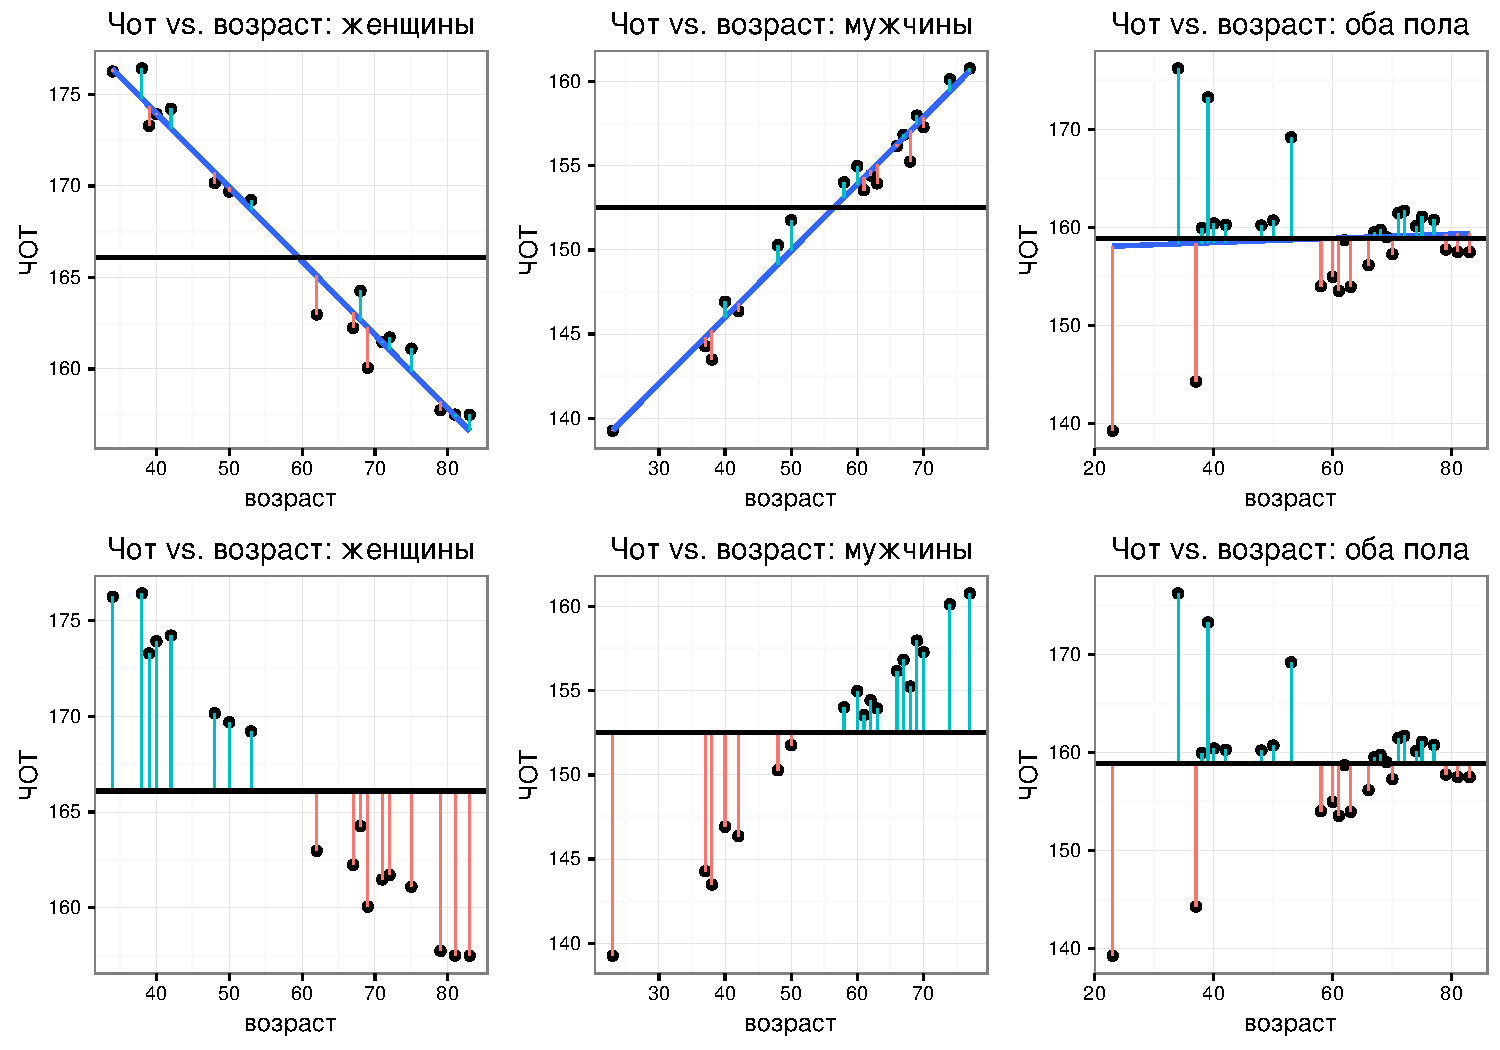
\includegraphics[width=0.9\linewidth]{r2.pdf}\\
\vfill
Во многих дисциплинах достаточно высокими считаются значения R² 0.5$\sim$ 0.6
\end{frame}

\begin{frame}{Как сравнить модели? AIC, BIC}
Для сравнения моделей используют несколько параметров:
\begin{itemize}
\mytem AIC — информационный критерий Акаике (чем меньше, тем лучше)\\
\scriptsize\verb"AIC()"\normalsize
\mytem BIC — байесовский информационный критерий Шварца (чем меньше, тем лучше)\\
\scriptsize\verb"BIC()"\normalsize
\end{itemize}
… надо сказать, разных вариантов этих критериев много, AIC и BIC —  самые популярные.
\end{frame}

\section{перебор моделей}
\begin{frame}{Перебор моделей}
Существует несколько стратегий перебора моделей:
\begin{itemize}
\mytem построить модель из всех предикторов, а потом "выкидывать" не значимые
\mytem строить модель снизу вверх добавляя по одному предиктору, выясняя какие значимы, а какие нет
\mytem смешанная
\end{itemize}
\vfill
Если много предикторов, то возникает желание перебрать все возможные варианты и узнать, в какой модели лучше скорректированный R², AIC и BIC. Для этого, естественно, уже написаны готовые функции (см. функцию \scriptsize\verb"step"\normalsize, \scriptsize\verb"regsubsets"\normalsize\ в пакете \scriptsize\verb"leaps"\normalsize, \scriptsize\verb"bestglm"\normalsize\ в пакете \scriptsize\verb"bestglm"\normalsize\ или пакет \scriptsize\verb"FWDselect"\normalsize\  и его описание \citep{sestelo2016}). Можно встретить отрицательное отношение к такой стратегии выискивания лучшей из моделей, построенных на одних и тех же данных, так как некоторые приравнивают ее к \textbf{\textit{data fishing}}.
\end{frame}
\begin{frame}{Перебор моделей: step}
Функция \scriptsize\verb"step"\normalsize перебирает модели на основе AIC. Аргумент \scriptsize\verb"direction"\normalsize позволяет выбрать стратегию перебора: \scriptsize\verb"backward"\normalsize, \scriptsize\verb"forward"\normalsize\ или \scriptsize\verb"both"\normalsize. По умолчанию функция показывает ход своей работы, чтобы вывести на экран характеристики выбранной модели, следует использовать функцию \scriptsize\verb"summary"\normalsize.
\vfill
\scriptsize
\begin{alltt}
step(lm(duration\textasciitilde., data = vowels))\\
step(lm(duration\textasciitilde., data = vowels), method = "both")\\
summary(step(lm(duration\textasciitilde., data = vowels), method = "both"))
\end{alltt}
\normalsize

\end{frame}

\section{другие регресии}
\begin{frame}{В данной презентации не рассказано о…}
\begin{itemize}
\mytem полиномиальной регрессии,
\mytem нелинейной регрессии,
\mytem логистической регрессии,
\mytem гребневой и лассо-регрессии,
\mytem и, наверное, о массе всего другого.
\end{itemize}
\end{frame}
\section{}
\begin{frame}
{\huge Спасибо за внимание\bigskip\\
\normalsize Пишите письма\\
agricolamz@gmail.com
\vspace{-130pt}}
\end{frame}
\begin{frame}{Список литературы}
\footnotesize
\bibliographystyle{chicago}
\bibliography{bibliography}
\end{frame}
\end{document}